
Como ya adelantamos brevemente en el apartado anterior, para la generación de oraciones para la síntesis utilizamos Festvox y Festival. Al igual que con las transcripciones fonéticas, estas herramientas nos permitirán traducir oraciones grafémicas (texto) a una lista de fonos y metadata utilizados por HTK para sintetizar audio.

El primer desafío que se presenta es que estos repertorios fonéticos no tienen un mapeo directo entre el inglés y el castellano: por ejemplo con el repertorio Fonético de Festvox en castellano, existen tres fonos distintos para la /i/, decisión que proviene de la necesidad de poder diferenciar la /i/ acentuada de la no acentuada  y de aquella presente en los diptongos: /ia/, /ie/, /io/, /iu/. La tabla \ref{fig:foneRep} muestra los repertorios utilizados por festvox para la generación de transcripciones fonéticas de castellano e ingles.

\begin{table}
\centering
%\setlength{\tabcolsep}{6pt} % default value is 6pt
\begin{minipage}[t]{0.3\textwidth}
\begin{tabular}[t]{cc}
\toprule
Castellano \\
\midrule
a & m \\
a1 & n \\
b & ny \\
ch & o \\
d & o1 \\
e & p \\
e1 & r \\
f & rr \\
g & s \\
i & sp \\
i0 & t \\
i1 & th \\
k & u \\
l & u0 \\
ll & u1 \\
 & x \\
\bottomrule
\end{tabular}
\end{minipage}
\begin{minipage}[t]{0.3\textwidth}
\begin{tabular}[t]{cc}
\toprule
Inglés \\ 
\midrule
 aa & jh\\
 ae & k \\
 ah & l \\
 ao & m \\
 aw & n \\
 ax & ng\\
 ay & ow\\
 b  &oy\\
 ch & p \\
 d  &r \\
 s  &sh\\
 dh & t\\
 eh & th \\
 er & uh \\
 ey & uw \\
 f  &v\\
 g  &w\\
 hh & y\\
 ih & z\\
 iy & zh \\
\bottomrule
\end{tabular}
\end{minipage}
\caption{Repertorios fonéticos utilizados por Festvox para inglés y castellano} 
\label{fig:foneRep}
\end{table}

%De aquí surgen varios problemas. El primero es que Festival utiliza el mismo símbolo para dos fonos distintos. De esta manera, la /g/ en castellano suena mucho mas disminuida que la /g/ del repertorio inglés, aunque ambas sean descritas como un fono oclusivo velar sonoro. Acá la cagué esto no era así =(.
%\cambiarEjemplo

De esto, surge el siguiente problema: cómo sintetizar oraciones en castellano utilizando un repertorio fonético en inglés, donde incluso la cantidad de fonos es diferente. La manera que encontramos de abordar esto fue confeccionar una tabla donde cada fono del castellano estuviera mapeado a uno del inglés. En otras palabras, antes del entrenamiento del modelo, tomamos los fonos generados por festival para el corpus en inglés y los reemplazamos con fonos del castellano de la manera ilustrada en la tabla 2.

\buscarEjemplosEl
\begin{table}
\centering
%\setlength{\tabcolsep}{6pt} % default value is 6pt
\caption{Mapeo Fonético}
\begin{minipage}[t]{0.3\textwidth}
\begin{tabular}[t]{c|c}
\toprule
Inglés & Castellano \\
\midrule
ae &	a \\
aa &	a1 \\
b &	b \\
ch &	ch \\
d &	d \\
dh &	d \\
eh &	e \\
el &	e1 \\
f &	f \\
hh & g \footnotemark\\
iy &	i \\
%falta  i0
ih &	i1 \\
k &	k \\
l &	l \\
jh &	ll \\
m &	m \\
n &	n \\
nx &	n \\
n + i &  ny \\
ao &	o \\
ou &	o1 \\
\bottomrule
\end{tabular}
\end{minipage}
\begin{minipage}[t]{0.3\textwidth}
\begin{tabular}[t]{c|c}
\toprule
Inglés & Castellano \\ 
\midrule
p &	p \\
r &	r/rr \\
%falta x
s &	s \\
t &	t \\
uw &	u \\
w &	u0 \\
uh &	u1 \\
g &	-\\
dx &- \\
em &- \\
en &- \\
er &- \\
ei &- \\
hv &- \\
ng &- \\
th &- \\
v & -\\
y & -\\
sh &- \\
zh &- \\
z & - \\ 

\bottomrule
\end{tabular}
\end{minipage}
\end{table}

\footnotetext{El mapeo de /hh/ a /g/ en castellano resultó ser incorrecto. El fono /g/ existe tanto en castellano (gato) como en ingles (glad). Notamos este error recién al hacer la evaluación perceptual, como se describe en la sección \ref{datosNormalizados}}

Por otro lado para varios fonos tuvimos que hacer reglas especiales ya que no contábamos con ningún fono del inglés lo suficientemente similar. Así,  para el fono ny (ñ o \textltailn, en ipa) colapsamos las apariciones del fono /n/ seguido de /i/. Si bien esta solución puede parecer algo forzada, ya que estamos generando de manera casera fonos a partir de otros, consideramos que esto se aproxima en cierta medida a la manera real en la que un hablante no nativo aprende un idioma con una carga fonética diferente al suyo. Citando un extracto del trabajo \textit{Transcription of Spanish and Spanish-Influenced English, Brian Goldstein, Temple University}\cite{spanishInfluencedEnglish}:

\begin{center}
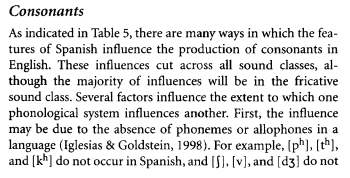
\includegraphics[scale=0.6]{imagenes_investigacion/consonantes1.png}
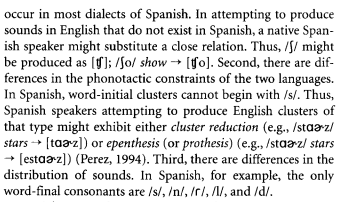
\includegraphics[scale=0.6]{imagenes_investigacion/consonantes2.png}
\end{center}

Visto desde nuestra perspectiva, una persona que aprende una nueva lengua, realiza una aproximación entre los fonos conocidos y los fonos `objetivo' de la nueva lengua.

Esta perspectiva nos alienta a realizar mapeos que no resultan del todo exacto, mapenado por ejemplo el fono /w/ (\textit{twentieth}) del ingles al fono /u0/ (\textit{ahuyentar}) del castellano o el fono /uw/ (\textit{two}) por el fono /u/ (\textit{cumplió}).

Un mapeo que podría resultar controversial es del fono /jh/ (\textit{danger}) del ingles por el /ll/ (\textit{billete}) del castellano. Si bien esta decisión no puede resultar ser la mejor, por ejemplo /ll/ podría ser mapeado a /sh/ (\textit{ash}), consideramos que para este primer trabajo resulta suficientemente buena.

De manera similar el inglés carece del fono vibrante múltiple alveolar sordo /\textipa{r}/ (\textit{perro}) y dado que el fono /\textipa{R}/(\textit{pero})  ya estaba siendo utilizado, no podíamos realizar un mapeo tan directo. Como solución tomamos la mitad de los fonos /\textipa{R}/ y los reemplazamos con /\textipa{r}/. 


Aquellos fonos que consideramos suficientemente disímiles del castellano, como es el caso de la /sh/, /z/, etc los mapeamos a caracteres que no interfirieran para el entrenamiento ya que no los utilizaremos para la síntesis de oraciones en castellano.


Con este mapeo, podemos utilizar solamente el corpus en ingles para sintetizar oraciones en castellano, aunque como es de esperar, dado que el corpus de entrenamiento es tan distinto de las oraciones que queremos sintetizar (Por cuestiones como que las combinaciones de fonos del ingles y el castellano son diferentes, las reglas prosódicas y las acentuaciones vocálicas difieren entre los idiomas) los audios sintetizados resultan incomprensibles.

% mapeo utilizado mostrar.
% el etiquetado de cmu\_arctic es en inglés y mapeando al castellano.